\chapter{Diskrete sannsynlighetsmodeller}
\label{kap:diskrete} % Opprinnelig kapittelnr: 2


Dette kapitlet gir en innføring i sannsynlighetsmodeller,
grunnleggende begreper og enkle regneregler for analyse basert på slike
 modeller.
\footnote{Appendiks  A gir en oversikt over noe av den
terminologi som vil bli brukt, og en ordliste norsk-engelsk.} 
For å ha en rød tråd gjennom temaene, vil vi tenke på et 
eksperiment med usikkert utfall, men id\'{e}ene kan overføres til
iakttakelser i andre sammenhenger.

\section{Eksperimenter med diskret utfallsrom}

\begin{center} \framebox[10cm]{\begin{minipage}{9cm} \rule{0cm}{0.5cm}
\begin{definisjon}
Mengden av alle mulige utfall av et eksperi\-ment
kalles {\em utfallsrommet} for eksperimentet.
\end{definisjon}
\end{minipage}} \end{center}

\noindent Vi krever av et utfallsrom at det skal være fullstendig og
skillende, dvs. at ett og bare ett av utfallene i utfallsrommet
inntreffer når eksperimentet utføres. Vi skal symbolisere et
utfallsrom med $\Omega$. Som generelt symbol for utfall bruker vi $u$.
 $\Omega$ er altså en mengde, og $u$ er element i $\Omega$, vi skriver
$u \in \Omega$ hvor symbolet $\in$ betyr ``er element i'',
Dersom antall utfall i utfallsrommet er enten endelig
eller tellbart uendelig, sier vi at utfallsrommet er $diskret$. I
dette kapitlet skal vi begrense oss til å studere eksperimenter
med diskret utfallsrom. I slike tilfeller kan vi liste opp
(nummerere) alle de mulige utfallene av eksperimentet, for
eksempel slik : $u_1, u_2, u_3,\ldots$
Utfallsrommet er da 

\[                      \Omega=\{u_1, u_2, u_3,\ldots\} \]
Når vi skal skrive ned et utfallsrom i en konkret situasjon, bør
vi representere hvert utfall med egnede symboler, for eksempel
med tall eller bokstaver. \\

\begin{eksempel}{Et myntkast}
Et egnet utfallsrom for et myntkast er $\Omega=\{K,M\}$ hvor
bokstavene $K$ og $M$ betegner henholdsvis kron og mynt. Nå
kunne det selvsagt tenkes at mynten ble stående på høykant.
For å fange inn denne muligheten kan en bruke utfallsrommet
$\Omega=\{K,M,H\}$, men $\Omega=\{K,M\}$ kan anses som
fullstendig for alle praktiske formål.
\end{eksempel}

\begin{eksempel}{Et terningkast}
Vi kaster en terning og ønsker å observere antall øyne. Et
eget utfallsrom er $\Omega=\{1,2,3,4,5,6\}$. Tallet 6
representerer 6 øyne etc.
\end{eksempel}

\begin{eksempel}{Loddtrekning}
Navnene på de $m$ studentene som er til stede på en forelesning
skrives ned på $m$ lapper. De $m$ lappene legges i en hatt og
blandes godt. En lapp skal trekkes ut tilfeldig, og navnet på
lappen registreres. Vi lar utfallsrommet være $\Omega=\{N_1,
N_2, \ldots,N_m\}$ hvor $N_1, N_2, \ldots,N_m$ er de $m$ navnene.
\end{eksempel}

\begin{eksempel}{Kvalitetskontroll}
En produsert artikkel kvalitetskontrolleres og klassifiseres i en
av to kate\-gorier intakt ($i$) eller defekt ($d$). Utfallsrom
$\Omega=\{i,d\}$. Dersom intakte artikler sorteres i tre
kvaliteter $a$, $b$ og $c$, vil $\Omega=\{a,b,c,d\}$ være et egnet
utfallsrom. Vi merker oss at utfallsrommet til et eksperiment
ikke nødvendigvis er entydig fastlagt ut fra eksperimentet, men
velges etter sitt formål.
\end{eksempel}

\begin{eksempel}{To myntkast}
En mynt kastes to ganger. Tre synspunkter kan gjøres gjeldene:
\begin{itemize}
\item  Det er to mulige utfall : Kastene viser likt ($\ell$), eller ulikt ($u$).
\item  Det er tre mulige utfall : Antall kron er enten 0, 1 eller 2.
\item Det er fire mulige utfall : Begge kastene viser kron,
     begge viser mynt, det første kastet viser kron og det andre
     mynt,det første kastet viser mynt, og det andre kron.
\end{itemize}
Vi har derfor minst tre mulige utfallsrom å velge mellom:
$\Omega_1=\{\ell, u\}$, $\Omega_2=\{0,1,2\}$ eller $\Omega_3=\{KK, KM,
MK, MM\}$. Av disse tre utfalls\-rommene vil en vanligvis
foretrekke det siste, blant annet fordi det, uten å være altfor
komplisert, er mest detaljert, og derfor kan fange opp flere
problemstillinger enn de to andre.
\end{eksempel}

     Det er langt fra et mål i seg selv å lage et mest mulig
detaljrikt utfalls\-rom. I Eksempel 1 kunne vi i tillegg til
resultatene kron eller mynt registrere med hvilken fart mynten
traff bordet, innfallsvinkelen, myntens plassering på bordet
etc. Alle slike ting er irrelevant i gambling og for en gambler
vil utfallsrommet $\Omega=\{K, M\}$ være detaljrikt nok.
Generelt kan man si at det er opp til brukeren å finne et
utfallsrom som passer til formålet. Utfallsrommet er 
referanserammen man velger å arbeide innenfor. \\

\noindent
{\bf Merknad} I Snorre's saga om Olav den hellige (94) forteller
Torstein Frode en historie der norske- og svenskekongen var enige
om å løse en tvist om et landområde ved kast med to terninger.
Etter gjentatte dobbel seksere vant til slutt norskekongen, da den ene
terningen ble kløvd på midten og viste (til sammen) syv! \\

\begin{eksempel}{Tre talere}
På et møte skal tre talere $A$, $B$ og $C$ holde hvert sitt
innlegg, og rekkefølgen skal bestemmes ved loddtrekning. Som
utfallsrom foreslås  $\Omega=\{ABC,\\ ACB, BAC, BCA, CAB, CBA\}$,
hvor $ABC$ betegner talerekkefølgen først $A$, deretter $B$ og
sist $C$, etc. Utfallsrommene har i alt 6 mulige utfall.
\end{eksempel}

\begin{eksempel}{Myntkast inntil første kron}
Vi skal kaste en mynt helt til vi får kron. Et mulig utfallsrom
er $\Omega=\{K, MK, MMK, MMMK,\ldots \}$. I denne situasjon vil det
være nok å regi\-strere antall kast som trengs for å få en
kron, et alternativt utfallsrom er derfor
$\Omega=\{1,2,3,4,\ldots \}$. Begge utfallsrom er tellbart uendelige.
Ethvert endelig utfallsrom vil være utilstrekkelig.
\end{eksempel}

\section{Diskrete sannsynlighetsmodeller}
\begin{center} \framebox[11cm]{\begin{minipage}{10cm} \rule{0cm}{0.5cm}
\begin{definisjon}
 Dersom vi har et eksperiment med diskret utfallsrom
$\Omega =\{u_1, u_2, u_3,\ldots\}$, og en funksjon $p$ som
tilfredstiller \\ \\
 $\mbox{\ \ \  A1.\ \ \ \ }   0 \leq p(u) \leq 1 \mbox{    for alle } u $\\ \\
 $\mbox{\ \ \  A2.\ \ \ \ }   p(u_1)+p(u_2)+p(u_3)+ \cdots =1 $ \\ \\
\noindent sier vi at $(\Omega, p)$ utgjør en {\em diskret
sannsynlighetsmodell} for eksperimentet. Funksjonen $p$ vil vi
kalle en {\em sannsynlighetsfunksjon}, og $p(u)$ vil vi kalle {\em
sannsynligheten} for utfallet $u$.
\end{definisjon}
\end{minipage}} \end{center}
Vi krever altså at sannsynligheten for hvert mulig utfall skal
være et reellt tall mellom 0 og 1 (begge skranker inkludert), og
at summen av sannsynlighetene for alle de mulige utfall skal være
1. La oss gi en motivering for denne definisjonen: Anta at vi har
gjentatt vårt eksperiment i alt $n$ ganger, og at vi har
observert $u_1, u_2, u_3,\ldots$ henholdsvis $n(u_1), n(u_2),
n(u_3),...$ ganger. Da er opplagt $0 \leq n(u)\leq n$ for alle
utfall $u$, og $n(u_1)+n(u_2)+n(u_3)+\cdots=n.$ Dividerer vi her
med $n$ får vi at de relative hyppighetene $h(u)=n(u)/n$ har
egenskapene $0\leq h(u)\leq 1$ for alle $u$, og
$h(u_1)+h(u_2)+h(u_3)+\cdots=1$. Siden vi ønsker et
sannsynlighetsbegrep som også skal betjene
forestillingen om sannsynligheter som idealiserte relative
hyppigheter (se Eksempel 1.1 og 1.2), må vi i hvert fall kreve A1 og A2.
\footnote{En del viktige formler er gitt navn A1, A2, A3,
E1, E2, etc. og er samlet gruppevis i Appendiks B.}

Som vi ser gir ikke vår definisjon noen anvisning på hvordan vi
eks\-plisitt skal beregne sannsynlighetene for hvert mulig utfall,
enhver funksjon $p: \Omega \rightarrow R$ som tilfredsstiller A1
og A2 er tillatt. Modellbyggeren står fritt til å velge en
sannsynlighetsfunksjon som samsvarer med de forestillinger
han/hun har om eksperimentet. \\

\begin{eksempel}{Et myntkast}
Utfallsrom $\Omega =\{K, M\}$. La oss skrive $p=p(K)$ og
$q=p(M)$. Her må ifølge krav A1 både $p$ og $q$ være tall mellom
0 og 1, og ifølge krav A2 må alltid $p+q=1$, dvs. $q=1-p$.
Forestillingen om at myntkastet er rettferdig uttrykkes i
modellen ved å sette $p=q=1/2$. Dersom det er grunn til å tro
mynten er ``skjev'', kan vi eksperimentere med mynten og basere
	modellen på den erfaring vi får. (Se Eksempel 1.2 og Oppgave~\ref*{kap:introduksjon}.1).
\end{eksempel}

\begin{eksempel}{Et terningkast}
Utfallsrom $\Omega =\{1,2,3,4,5,6\}$. Forestillingen om en
rettferdig terning svarer i en modell til at alle de 6 utfallene
er like sannsynlige, dvs. $p(1) = p(2) = p(3) = p(4) = p(5) =
p(6) = p$. På grunn av A2 må derfor $p+p+p+p+p+p=6\cdot p=1$, som
gir at $p=1/6$. Dersom vi ikke uten videre vil anta
at terningen er rettferdig, kan vi skaffe kunnskap ved å
eksperimentere med den. Anta at vi i løpet av $n=1000$ kast 
observere $n(1) = 194, n(2) = 166, n(3) = 177, n(4) = 181, n(5) =
150, n(6) = 132$. På bakgrunn av denne erfaring er følgende
sannsynlighetsfunksjon aktuell (se også Oppgave~8):
\begin{eqnarray*}
     p(1) = 0.19,& p(2) = 0.17,& p(3) = 0.18 \\ 
     p(4) = 0.18,& p(5) = 0.15,& p(6) = 0.13
\end{eqnarray*}
\noindent Vårt eksperiment har imidlertid ikke bevist at terningen er
falsk. Erfaring viser at de tilfeldige variasjoner i terningkast
er store, og resultatet kan derfor godt skyldes tilfeldigheter.
Er det observerte resultat tilstrekkelig ekstremt til å vrake
modellen om rettferdighet? Statistisk teori besvarer slike
spørsmål.
\end{eksempel}

\begin{eksempel}{Loddtrekning}
Utfallsrom $\Omega = \{N_1, N_2, \ldots, N_m\}$. En rettferdig
trekning er en trekning der alle lapper har samme sannsynlighet
for å bli trukket ut. En modell for en rettferdig trekning er
derfor gitt ved
\[  p(N_1) = p(N_2) = \cdots = p(N_m) = 1/m \]
\end{eksempel}

\begin{eksempel}{To myntkast}
Utfallsrom $\Omega =\{KK, KM, MK, MM\}$. En mulig modell 
antar at alle fire utfall er like sannsynlige, dvs. $p(KK) = p(KM)
= p(MK) = p(MM) = 1/4$.
\end{eksempel}

\begin{eksempel}{Myntkast inntil første kron}
Utfallsrom $\Omega =\{1,2,3,4,\ldots   \}$. Siden
${\frac{1}{2}}+{(\frac{1}{2})}^2+{(\frac{1}{2})}^3+{(\frac{1}{2})}^4+\cdots 
=1$ , er sannsynlighetsfunksjonen $p$ gitt ved $p(1)={\frac{1}{2}}$,
$p(2)={(\frac{1}{2})}^2$, $p(3)={(\frac{1}{2})}^3$,\\ $p(4)={(\frac{1}{2})}^4$,
 \ldots , dvs. $p(n)={(\frac{1}{2})}^n$, $n=1,2,3,4, \ldots$ en aktuell
kandidat. Vi skal senere vise
at rimelige antagelser om eksperimentet nettopp leder til denne
modellen. Merk at denne modellen innebærer at muligheten for å
vente i det uendelige på kron ikke er tilstede, dvs. er tildelt
sannsynlighet null.
\end{eksempel}

\section{Begivenheter}

\begin{center} \framebox[11cm]{\begin{minipage}{10cm} \rule{0cm}{0.5cm}
\begin{definisjon}
 Enhver delmengde $A$ av utfallsrommet $\Omega$ kalles en {\em begivenhet}.
 De utfall begivenheten $A$ er sammensatt av kalles {\em gunstige
utfall} for $A$. Vi sier at begivenheten $A$ har inntruffet hvis og
bare hvis et av de gunstige utfall for $A$ har inntruffet.
\end{definisjon}
\end{minipage}} \end{center}
Begrepet begivenhet er innført fordi vi ofte ønsker å gi en
mindre detaljrik beskrivelse av et eksperimentresultat enn den
hvert utfall gir.  En begivenhet $A$
kan beskrives enten ved at vi lister opp de utfall $A$ er
sammensatt av, eller ved at vi gir en verbal beskrivelse i form
av en egenskap som kjennetegner de og bare de utfall som er med i $A$.

Merk at ifølge vår definisjon er utfallsrommet $\Omega$ også
en begivenhet. $\Omega$ er nødt til å inntreffe, og vi gir derfor
$\Omega$ navnet {\em den sikre begivenhet}. Den tomme mengde
$\emptyset$ er også en begivenhet. Siden intet utfall er gunstig for
$\emptyset$, kalles denne for {\em den umulige begivenhet}. En
begivenhet som består av bare ett utfall kaller vi en {\em enkel
begivenhet}, en begivenhet som består av mer enn ett utfall kaller
vi en {\em sammensatt begivenhet}. Vi vil vanligvis benytte store bokstaver
 fra begynnelsen av alfabetet som symboler  på begivenheter.\\

 \begin{eksempel}{To myntkast}
 Utfallsrom $\Omega =\{KK, KM, MK, MM\}$. Her er en liste over
 alle tenkelige delmengder av $\Omega$ : \\[1mm]
 \noindent $B_1 = \{KK\}, B_2 = \{KM\}, B_3 = \{MK\}, B_4 = \{MM\}, B_5 =
 \{KK, KM\},\\ B_6 = \{KK, MK\}, B_7 = \{KK, MM\}, B_8 = \{KM, MK\},
 B_9 = \{KM, MM\},\\ B_{10} = \{MK, MM\}, B_{11} = \{KK, KM, MK\}, B_{12}
 = \{KK, KM, MM\},\\ B_{13} = \{KK, MK, MM\}, B_{14} = \{KM, MK, MM\},
 B_{15} = \Omega , B_{16} = \emptyset $.\\[1mm]
 Det er i alt $16 = 2^4$ ulike delmengder (begivenheter) i $\Omega$.
 Eksempler på verbale beskrivelser: $B_5 =$ første kast gir kron,
 $B_9 =$ annet kast gir mynt, $B_4 =$ ingen kron, $B_7 =$ begge
 kast gir det samme, $B_{11} =$ minst et kast gir kron. Her er $B_1$
 til og med $B_4$ enkle begivenheter, mens $B_5$ til og med $B_{15}$
 er sammensatte begivenheter. Eksempelvis vil tre kron være den
 umulige begivenhet.
 \end{eksempel}

 Gitt en diskret sannsynlighetsmodell $(\Omega , p)$ for et
 eksperiment. Sannsynligheten $p(u)$ for hvert utfall $u\in
 \Omega$ er da fastlagt. Vi ønsker også å snakke om
 sannsynligheten til en vilkårlig begivenhet $A$ i utfallsrommet,
 kall denne for $P(A)$. \\

 \begin{center} \framebox[11cm]{\begin{minipage}{10cm} \rule{0cm}{0.5cm}
 \begin{definisjon}
      {\em Sannsynligheten til begivenheten} $A$ er
      summen av sannsynlighetene for de gunstige utfall for $A$,
      dvs. med symboler
 \[ \mbox{\ \ \  A3.\ \ \ \ \ \ }   P(A)=\sum_{u \in A}p(u) \]
 \noindent  hvor summasjonen går over alle utfall med i $A$.
 \end{definisjon}
 \end{minipage}} \end{center}



\noindent Symbolkombinasjonen $\sum_{u \in A}$ betyr summen av de ledd hvor $u$
er med i $A$, eksempelvis dersom $A = \{u_1, u_2, u_4, u_7\}$, så er

\[  P(A)=\sum_{u \in A}p(u)=p(u_1)+p(u_2)+p(u_4)+p(u_7) \]

\begin{eksempel}{To myntkast}
Modellen som er foreslått i Eksempel 11 gir eksempelvis
 $P(B_5)=p(KK)+p(KM)=\frac{1}{4}+\frac{1}{4}=\frac{1}{2}$,
 $P(B_9)=p(KM)+p(MM)=\frac{1}{4}+\frac{1}{4}=\frac{1}{2}$,\\[1mm]
 $P(B_4)=p(MM)=\frac{1}{4}$,
 $P(B_7)=p(KK)+p(MM)=\frac{1}{4}+\frac{1}{4}=\frac{1}{2}$,\\[1mm]
 $P(B_{11})=p(KK)+p(KM)+p(MK)=\frac{1}{4}+\frac{1}{4}+\frac{1}{4}=\frac{3}{4}$.
\end{eksempel}

\begin{eksempel}{Ventetid til første kron i myntkast}
Utfallsrom $\Omega = \{1,2,3,4, \ldots \}$. La $A = \{4,5,6,7,8, \ldots \}
=$ første kron kommer i fjerde kast eller senere og $B =
\{1,3,5,7,9, \ldots \} =$ første kron kommer etter et odde antall
kast. Den foreslåtte modell gir 
$P(A)=p(4)+p(5)+p(6)+\cdots ={(\frac{1}{2})}^4+{(\frac{1}{2})}^5+
{(\frac{1}{2})}^6+ \cdots ={(\frac{1}{2})}^4 \cdot {(1-{\frac{1}{2}})}^{-1}=
\frac{1}{8}$ og $P(B)=p(1)+p(3)+p(5)+\cdots =\frac{1}{2}+{(\frac{1}{2})}^3+
{(\frac{1}{2})}^5+ \cdots =\frac{1}{2} \cdot {(1-{\frac{1}{4}})}^{-1}=
\frac{2}{3}$
 ved bruk av summeformelen for en uendelig geometrisk rekke.
 \footnote{En uendelig geometrisk rekke er en sum av form
     $a+ar+ar^2+ar^3+\cdots$
dvs. der etterfølgende ledd alltid er r ganger det foregående.
Dersom r i tallverdi er mindre enn 1, blir summen av rekken lik
$a(1-r)^{-1}$, dvs. første ledd dividert med en minus forholdstallet.}
\end{eksempel}

Vi merker oss at dersom $E = \{u\}$ er en enkel begivenhet, så
gir defini\-sjonen at $P(E) = p(u)$. Vi er derfor fristet til å la
være å skille mellom et utfall $u$ og den tilhørende enkle
begivenhet $E = \{u\}$, og å benytte samme symbol, stor $P$, for
alle sannsynligheter.

For å gjøre det mulig å regne med begivenheter skal vi nå
 innføre mengdeoperasjonene union, snitt og komplement. \\

\begin{figure}[ht]
\centering \centering
 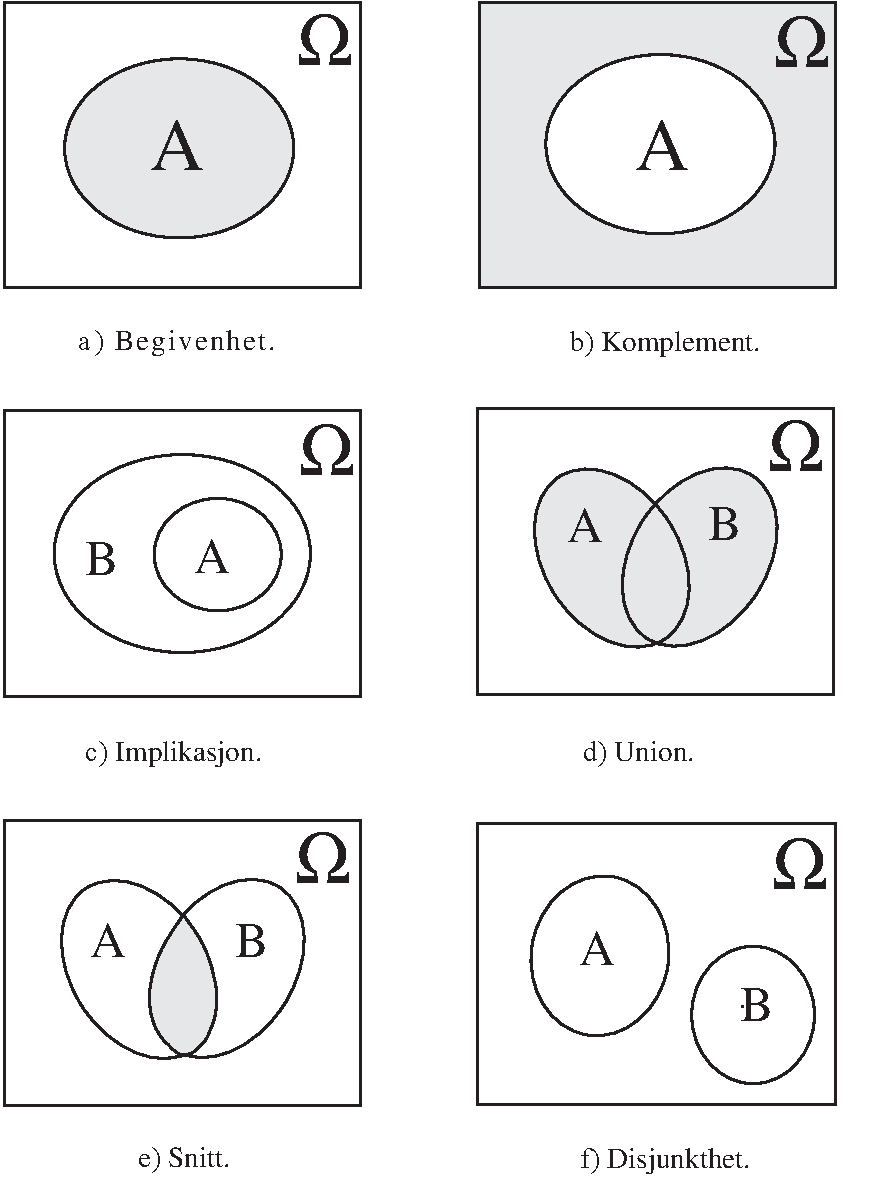
\includegraphics[scale=0.7]{figurer/fig2_1.pdf}
 \caption{Elementer i mengdelære}
	\label{fig:mengdelare}
\end{figure}
\clearpage

\begin{center} \framebox[11cm]{\begin{minipage}{10cm} \rule{0cm}{0.5cm}
\begin{definisjon}{\em Unionen} av begivenhetene $A$ og
     $B$ skriver vi $A \cup B$, og er den begivenhet som består
     av alle utfall som enten er med i $A$ eller med i $B$ (eller
     med i både $A$ og $B$).
\end{definisjon}
\end{minipage}} \end{center}
\noindent Vi ser at begivenheten $A \cup B$ har inntruffet hvis og bare
hvis enten $A$ eller $B$ (eller begge) har inntruffet. Derfor
blir $A \cup B$ ofte kalt ``begivenheten $A$ eller $B$''.

\begin{center} \framebox[11cm]{\begin{minipage}{10cm} \rule{0cm}{0.5cm}
\begin{definisjon}
     {\em Snittet} av begivenhetene $A$ og
     $B$ skriver vi $A \cap B$, og er den begivenhet som består
     av de utfall som både er med i $A$ og med i $B$.
\end{definisjon}
\end{minipage}} \end{center}
\noindent Vi ser at begivenheten $A \cap B$ har inntruffet hvis og bare
hvis både $A$ og $B$ har inntruffet. Derfor blir $A \cap B$ ofte
kalt ``begivenheten $A$ og $B$''. Dersom $A$ og $B$ ikke har
noe utfall felles, er $A \cap B$ lik den umulige begivenhet
$\emptyset$. I så fall sier vi at $A$ og $B$ er {\em disjunkte
begivenheter}. To begivenheter som er disjunkte kan altså ikke
begge inntreffe.

\begin{center} \framebox[11cm]{\begin{minipage}{10cm} \rule{0cm}{0.5cm}
\begin{definisjon}
     {\em Komplementet} til begivenheten
     $A$, skriver vi $\bar{A}$, og er den begivenhet som består av alle
     utfall i ut\-fall\-srommet som ikke er med i $A$.
\end{definisjon}
\end{minipage}} \end{center}
\noindent Vi ser at begivenheten $\bar{A}$ har inntruffet hvis og bare hvis
begivenheten $A$ ikke har inntruffet. Derfor blir $\bar{A}$ ofte kalt
``begivenheten ikke-$A$''.
\footnote{Mange foretrekker isteden skrivemåten $A^c$ for å unngå
at $\bar{A}$ forveksles med notasjon for gjennomsnitt.}

\begin{center} \framebox[11cm]{\begin{minipage}{10cm} \rule{0cm}{0.5cm}
\begin{definisjon} Vi sier at $A$ er {\em delmengde} av
     $B$, og skriver $A \subset B$, dersom ethvert utfall i $A$
     også er med i $B$.
\end{definisjon}
\end{minipage}} \end{center}
\noindent Når $A \subset B$, så vil, dersom $A$ har inntruffet,
også $B$ ha inntruffet. Vi sier at begivenheten $A$ {\em impliserer}
(medfører) begivenheten $B$. De innførte begreper illustreres
gjerne ved å tenke seg begivenheter (mengder) representert ved
områder i planet, såkalte {\em Venn-diagrammer}, se figurene 1-6.



I Figur~\ref{fig:mengdelare}a er begivenheten $A$ skravert, i Figur~\ref{fig:mengdelare}b begivenheten
$\bar{A}$. Figur~\ref{fig:mengdelare}c illustrerer utsagnet $A \subset B$. I Figur~\ref{fig:mengdelare}d er
begivenheten $A \cup B$ skravert, og i Figur~\ref{fig:mengdelare}e er $A \cap B$
skravert. Figur~\ref{fig:mengdelare}f illustrerer utsagnet $A \cap B = \emptyset$.\\


\begin{eksempel}{Et terningkast}
Utfallsrom $\Omega =\{1,2,3,4,5,6\}. A =\{4,5,6\} =$ minst fire
øyne, $B = \{3,6\} =$ antall øyne delelig med tre, $C = \{1,2\}
=$ høyst to øyne, er alle begivenheter. Her er $\bar{A} = \{1,2,3\} =$
høyst tre øyne, $A \cup B = \{3,4,5,6\} =$ minst tre øyne, $A
\cap B = \{6\} =$ seks øyne, $B \cap C = \emptyset $ og $C \subset \bar{A}$.
\end{eksempel}

\noindent Av og til trenger vi å snakke om unioner og snitt av mer enn to
begivenheter: La $B_1, B_2,\ldots , B_n$ være $n$ begivenheter. Den
begivenhet som består av de utfall som er med i minst en av
$B_i$'ene, kaller vi {\em unionen} av de $n$ begivenhetene, og vi
skriver $B_1 \cup B_2 \cup \ldots \cup B_n$ eller kortere  $\cup_{i=1}^{n}B_i$.
Den begivenhet som består av de utfall som er med i alle
$B_i$`ene kaller vi {\em snittet} av de $n$ begivenhetene, og vi
skriver $B_1 \cap B_2 \cap \ldots \cap B_n$ eller kortere  $\cap_{i=1}^{n}B_i$.
På tilsvarende måte defineres union og snitt av en uendelig følge
av begivenheter, med skrivemåte henholdsvis  $\cup_{i=1}^{\infty}B_i$ og
$\cap_{i=1}^{\infty}B_i$  . \\

\begin{eksempel}{Rakettoppskyting}
I et forskningsprogram skal det skytes opp $n$ raketter, hver
oppskyting blir enten suksess eller fiasko. Anta at vi i en
modell for resultatet av hele programmet, har definert $n$
begivenheter $A_1, A_2, \ldots, A_n$, hvor $A_i$ er begivenheten
at oppskyting nr. i er suksess. Her blir \\[1mm]
$B = A_1 \cup A_2 \cup \cdots \cup A_n$
    begivenheten at minst en oppskyting er suksess,\\
$C = A_1 \cap A_2 \cap \cdots \cap A_n$ begivenheten at alle     
                                   oppskytingene er suksess,\\
$D = \bar{A}_1 \cup \bar{A}_2 \cup \cdots \cup \bar{A}_n$
 begivenheten at minst en  oppskyting er fiasko, og \\
$E = \bar{A}_1 \cap \bar{A}_2 \cap \cdots \cap \bar{A}_n$
 begivenheten at alle oppskytingene er fiasko.\\[1mm]
Vi innser lett at $\bar{B} = E$ og $\bar{C} = D$.
\end{eksempel}

De sammenhenger vi oppdager i Eksempel 17 gjelder generelt og
kalles {\em De Morgans lover}\index{De Morgans lover}. Disse lyder altså

\begin{center} \framebox[10cm]{\begin{minipage}{9cm} \rule{0cm}{0.5cm}
{\bf De Morgans lover}: \\ \\
 $ \mbox{\ \ \  M1.\ \ \ \ }  \overline{A_1 \cup A_2 \cup \cdots \cup A_n}=
   \bar{A}_1 \cap \bar{A}_2 \cap \cdots \cap \bar{A}_n$ \\ \\
 $ \mbox{\ \ \  M2.\ \ \ \ }  \overline{A_1 \cap A_2 \cap \cdots \cap A_n}=
   \bar{A}_1 \cup \bar{A}_2 \cup \cdots \cup \bar{A}_n$  \\ \\
\end{minipage}} \end{center}
\noindent Forsøk å bli overbevist om at M1 og M2 gjelder generelt, for
eksempel ved å gi en verbal (ikke, og, eller) fortolking av
venstre- og høyresiden i hver likhet, eller ved å tegne 
Venn-diagrammer for tilfellet med bare to begivenheter (Oppgave~15).

For senere referanser nevner vi til slutt i dette avsnittet at en
følge $B_1, B_2, B_3,\ldots$ av begivenheter sies å være {\em
disjunkte} dersom $B_i \cap B_j = \emptyset$ for alle $i \neq j$, dvs.
dersom aldri to av begivenhetene kan inntreffe samtidig.
Illustrer at de tre begivenhetene $B_1$, $B_2$ og $B_3$ er
disjunkte med et Venn-diagram!


\section{Egenskaper ved sannsynligheter}

Av de tre aksiomene A1, A2 og A3 for sannsynligheter kan vi nå
avlede en rekke fundamentale egenskaper: Først to egenskaper som
innses direkte:

\begin{center} \framebox[10cm]{\begin{minipage}{9cm} \rule{0cm}{0.5cm}
 $ \mbox{\ \ \  E1.\ \ \ \ } 0 \leq P(A) \leq 1 \mbox{    for alle begivenheter  } A $ \\ \\
 $ \mbox{\ \ \ \ E2.\ \ \ \ }    P(\Omega)=1 $ \\ 
\end{minipage}} \end{center}
\noindent eller sagt med ord: En sannsynlighet er alltid et reelt tall
mellom 0 og 1 (begge skranker inkludert), og sannsynligheten for
den sikre begivenhet er 1. Så følger den viktige \\

\begin{center} \framebox[11cm]{\begin{minipage}{10cm} \rule{0cm}{0.5cm}
{\bf Addisjonssetningen for disjunkte begivenheter:} \\ \\
 $\mbox{\ \ \  E3.\ \ \ \ } P(A \cup B) = P(A) + P(B)  \mbox{  når \ } A \cap B = \emptyset $ \\ 
\end{minipage}} \end{center}
\noindent eller sagt med ord: Dersom begivenhetene $A$ og $B$ er disjunkte
(ikke kan inntreffe samtidig), så er sannsynligheten for
begivenheten $A$ eller $B$ lik sannsynligheten for $A$ pluss
sannsynligheten for $B$. \\                                 

\noindent Begrunnelse: Siden $A$ og $B$ ikke har noe utfall felles blir
\begin{center}
\begin{tabular}{ccc}
 $P(A \cup B)$&$=$& sum av sannsynlighetene for alle utfall i $A \cup B$ \\
           &$=$& sum av sannsynlighetene for utfallene i $A$ \\
           &$+$& sum av sannsynlighetene for utfallene i $B$ \\
           &$=$& $P(A) + P(B)$.
\end{tabular}
\end{center}
\noindent Siden $A \cup \bar{A} = \Omega$ og $A \cap \bar{A} = \emptyset$,
 får vi av E2 og E3 at $1 = P(\Omega) = P(A \cup \bar{A}) = P(A) + P(\bar{A})$. Dette gir

\begin{center} \framebox[10cm]{\begin{minipage}{9cm} \rule{0cm}{0.5cm}
 $ \mbox{\ \ \  E4.\ \ \ \ \ \ \ \ \ \ }   P(\bar{A}) = 1-P(A) $ \\
\end{minipage}} \end{center}
\noindent Siden komplementet til $\Omega$ er $\emptyset$ får vi spesielt av E2 og E4 at

\begin{center} \framebox[10cm]{\begin{minipage}{9cm} \rule{0cm}{0.5cm}
 $  \mbox{\ \ \  E5.\ \ \ \ \ \ \ \ \ \ \ }  P(\emptyset) = 0 $ \\ 
\end{minipage}} \end{center}
dvs. sannsynligheten for den umulige begivenhet er null.
Merk at E4 og E5 også kan fås av A3 direkte. En mengdefunksjon $P$
som har egenskapene E1, E2 og E3 (og derfor også E4 og E5) kalles
ofte et {\em sannsynlighetsmål}.

     E3 og E4 er svært nyttige når en skal løse
 sannsynlighetsteoretiske oppgaver i praksis. Ofte kan en
begivenhet som en ønsker å beregne sannsynligheten for, uttrykkes
som en disjunkt union av begivenheter med kjente sannsynligheter,
eller som et komplement av en begivenhet med kjent sannsynlighet.
Her er et eksempel som illustrerer begge bruksmåter: \\

\begin{eksempel}{Maskindeler}
Gitt at en masseprodusert maskindel blir for lang med
sannsynlighet 0.08, for kort med sannsynlighet 0.04. Vi ønsker å
beregne sannsynligheten for C = hverken for kort eller for lang.
Vi ser at begivenhetene A = for lang og B = for kort er
disjunkte, og at $\bar{C} = A \cup B$. Vi får da
\begin{eqnarray*}
    P(C)& = & 1 -P(\bar{C}) = 1-P(A \cup B) \\
        & = & 1 -(P(A) + P(B)) \\
        & = & 1 -(0.08 + 0.04) = 0.88 
\end{eqnarray*}
\end{eksempel}
\noindent Av og til vil vi trenge følgende generalisering av E3: \\
\begin{center} \framebox[10cm]{\begin{minipage}{9cm} \rule{0cm}{0.5cm}
{\bf Den generelle addisjonssetningen :} \\ \\
 $ \mbox{\ \ \  E6.\ \ \ \ }  P(A \cup B) = P(A) + P(B) - P(A \cap B) $ \\ 
\end{minipage}} \end{center}
\noindent Tar vi summen av sannsynlighetene for alle utfall i $A \cup B$,
ved å legge sammen sannsynlighetene for utfallene i $A$ og i $B$
hver for seg, ser vi av Figur~\ref{fig:mengdelare}d at utfallene i $A \cap B$ blir
tatt med to ganger, og vi korrigerer derfor for dette ved å
trekke fra $P(A \cap B)$. Dersom $A \cap B = \emptyset$, vil $P(A \cap B)
= P(\emptyset) =0$, og vi har fått tilbake addisjonssetningen for
disjunkte begivenheter. \\

\begin{eksempel}{Nøkkelpersonene}
Arnesen og Bjørnsen er de eneste som har nøkkel til pengeskapet i
sitt firma. Anta definert begivenhetene $A$ = Arnesen er til stede,
$B$ = Bjørnsen er til stede, $C$ = begge er til stede, $D$ = minst en
er til stede og $E$ = ingen er til stede. Gitt at $P(A)$ = 0.80,
 $P(B)$ = 0.70 og $P(C)$ = 0.56. Kan vi nå finne $P(D)$ og $P(E)$?
Vi ser at $C = A \cap B$, $D = A \cup B$ og $E =\bar{A}\cap \bar{B} = \bar{D}$.
 Vi får $P(D) = P(A \cup B) = P(A) + P(B) -P(A \cap B) = 0.80 + 0.70
- 0.56 = 0.94$  og  $P(E) = P(\bar{D}) = 1 - P(D) = 1 - 0.94 = 0.06$.
\end{eksempel}

\noindent Vi kan generalisere E3 i en annen retning, nemlig \\
\begin{center} \framebox[11cm]{\begin{minipage}{10cm} \rule{0cm}{0.5cm}
 Dersom $A_1, A_2, \ldots, A_n$ er $n$ disjunkte
begivenheter, så er \\ \\
 $\mbox{\ \  E7.\ \ \ \ } P(A_1 \cup A_2 \cup \cdots \cup A_n) =
                  P(A_1) + P(A_2) + \cdots + P(A_n) $ \\ 
\end{minipage}} \end{center}  

\noindent Dette resultatet kan vises på samme måte som E3.


\section{Uniforme sannsynlighetsmodeller}

La $\Omega = \{u_1, u_2, \ldots, u_m \}$ være et utfallsrom med
et endelig antall utfall $m$. \\
\begin{center} \framebox[11cm]{\begin{minipage}{10cm} \rule{0cm}{0.5cm}
\begin{definisjon}
 En sannsynlighetsmodell der alle $m$ utfall har samme sannsynlighet
 kaller vi en {\em uniform sannsynlighetsmodell}.
\end{definisjon}
\end{minipage}} \end{center}
\noindent La oss se hva som generelt karakteriserer slike modeller : Siden
nå $P(u_1) = \cdots = P(u_m) = p$, får vi av A2 at

\[ 1 = P(u_1) + P(u_2) + \cdots + P(u_m) = p+p+ \cdots +p = m \cdot p \]

\noindent Herav følger at $p = 1/m$, dvs. i en uniform modell er
sannsynligheten $p$ for hvert utfall lik en dividert med antall
mulige utfall. La oss finne sannsynligheten for en vilkårlig
begivenhet $A$. Anta at $A$ består av i alt $g$ gunstige utfall. Ifølge
A3 blir

\[     P(A)=\sum_{u \in A}P(u)=\sum_{u \in A}\frac{1}{m}=
                     g \cdot \frac{1}{m}= \frac{g}{m} \]

\noindent Av dette kan vi trekke en vidtrekkende konklusjon, nemlig
\begin{center} \framebox[11cm]{\begin{minipage}{10cm} \rule{0cm}{0.5cm}
     {\bf Regelen om ``gunstige på mulige'' :} I en uniform
     sannsynlighetsmodell kan sannsynligheten for enhver
     begivenhet $A$ finnes ved å dividere antall gunstige utfall
     for $A$ med antall mulige utfall i utfallsrommet $\Omega$.\\
\end{minipage}} \end{center}
\noindent Dette viser at uniforme sannsynlighetsmodeller vil være spesielt
enkle å arbeide med. Dersom det eksperimentet vi studerer
inneholder visse symmetrier, kan det lønne seg å utnytte dette
ved valg av utfallsrom og modell. Vi har sett eksempler på
uniforme modeller i eksemplene 8,9,10 og 11 ovenfor.\\

\begin{eksempel}{Korttrekning}
En vanlig kortstokk inneholder 52 kort: 13 spar, 13 hjerter, 13
ruter og 13 kløver. Den stokkes godt, og et kort trekkes
tilfeldig. Her er det rimelig å velge en uniform modell. Det er i
alt $m$ = 52 mulige utfall, og hvert utfall får da sannsynlighet
1/52. Vi er interessert i sannsynlighetene for begivenhetene $A$ =
rødt kort, $B$ = hjerter, $C$ = hjerter dame, $D$ = dame og $E$ = honnør
(ess, konge, dame, knekt). Antall gunstige utfall for disse
begivenheter er henholdsvis 26, 13, 1, 4 og 16. Vi får derfor
%\begin{center}
\begin{tabular}{lll}
 $P(A)=\frac{26}{52}=\frac{1}{2}$,&$P(B)=\frac{13}{52}=\frac{1}{4}$,
                               &$P(C)=\frac{1}{52}$ \\[1mm]
 $P(D)=\frac{4}{52}=\frac{1}{13}$,&$P(E)=\frac{16}{52}=\frac{4}{13}$&      
\end{tabular}
%\end{center}
\end{eksempel}
\begin{eksempel}{To terningkast}
En terning skal trilles to ganger (eller to terninger en gang).
Vi ønsker bl.a. å uttale oss om sannsynligheten for at sum øyne
på de to terningene blir syv. Velger vi $\Omega = \{ 2,3,4, \ldots ,
11, 12\}$ som utfallsrom (utfall er sum øyne), og antar uniform
modell, vil hvert utfall få tildelt sannsynlighet 1/11. Vår
intuisjon sier imidlertid at det må være mye lettere å oppnå 7
enn 12, og denne modellen er trolig svært urealistisk. Det er
ikke uten videre lett å innse hvilke sannsynligheter vi bør
tildele hvert utfall i dette utfallsrommet. La oss i stedet velge
et utfallsrom $\Omega$ med følgende utfall:
\begin{center}
\begin{tabular}{cccccc}
(1,1)&(1,2)&(1,3)&(1,4)&(1,5)&(1,6) \\
(2,1)&(2,2)&(2,3)&(2,4)&(2,5)&(2,6) \\
(3,1)&(3,2)&(3,3)&(3,4)&(3,5)&(3,6) \\
(4,1)&(4,2)&(4,3)&(4,4)&(4,5)&(4,6) \\
(5,1)&(5,2)&(5,3)&(5,4)&(5,5)&(5,6) \\
(6,1)&(6,2)&(6,3)&(6,4)&(6,5)&(6,6) \\
\end{tabular}
\end{center}
(1,6) betegner første terning viser 1, den andre 6 osv. Her er
det av symmetrigrunner, såframt terningen(e) er rettferdig(e),
rimelig å bruke en uniform modell. Hvert utfall får da tildelt
sannsynlighet 1/36. Her blir begivenheten $A$ = sum øyne lik syv
$=\{(1,6), (2,5), (3,4), (4,3), (5,2), (6,1)\}$. Som vi ser er
det 6 gunstige utfall for $A$. Bruker vi regelen om ``gunstige på
mulige'' gir modellen at sannsynligheten for $A$ er lik $P(A) = g/m
= 6/36 = 1/6$. På samme måte kan vi nå besvare en rekke andre
sannsynlighetsteoretiske spørsmål vedrørende dette eksperimentet
(Oppgave~18).
\end{eksempel}

I dette avsnittet har vi altså sett at beregning av
sannsynligheter i en uniform modell kan reduseres til et
telleproblem. Som vi snart skal se, vil det ikke alltid være like
lett å foreta opptellingen som i eksemplene ovenfor. I mer
kompliserte problemstillinger vil ofte de kombinatoriske metodene
som vi skal presentere i neste kapittel være til hjelp.


\section{Oppgaver}
\small
\begin{enumerate}
\item  Eva skal føde. Diskuter valg av utfallsrom.
\item  Familien som skal flytte inn i leiligheten ved siden av Per
     har et barn som skal begynne på samme skole som han. Per er
     spent på kjønn og klassetrinn (1 til 6). Foreslå et egnet
     utfallsrom når vi ønsker å holde rede på både kjønn      og klassetrinn.
\item  Foreslå et egnet utfallsrom for en to-barns-familie.
\item  En student velges ut fra en gruppe av studenter og blir
     spurt om hvor mange søsken han/hun har. Foreslå et passende
     utfallsrom.
\item  Antall oppringninger til et sentralbord i et gitt tidsrom
     skal behandles som et stokastisk fenomen. Foreslå et
     passende utfallsrom.
\item  En urne inneholder tre kuler, en rød, en hvit og en blå. To
     kuler trekkes ut etter tur. Foreslå et egnet utfallsrom når\\[1mm]
     (a)  vi tar omsyn til rekkefølgen av de uttrukne kulene.  \\
     (b)  vi ikke tar omsyn til dette.\\
     Anta at den uttrukne kule blir lagt tilbake i urnen før
     annen trekning foretas. Besvar (a) og (b) også under denne
     forutsetningen.
\item  Fire personer skal avgjøre hvilket produkt x eller y  de
     liker best. Foreslå et egnet utfallsrom når vi ønsker å
     holde rede på hvem som valgte hva.
\item  En terning hvor 1 og 6 er motstående sider er fikset ved å
     plassere et lite lodd inne i terningen ved midten av sekser-
     siden. Lag en sannsynlighetsmodell for et terningkast med
     terningen når n = 1000 kast ga de resultatene som er gitt i
     Eksempel 9, og vi antar at utfallene 2,3,4,5 fortsatt er like
     sannsynlige.
\item  En falsk terning er laget ved at enersiden er høvlet ned
     litt. Lag en sannsynlighetsmodell for et terningkast med
     denne terningen når n = 1000 kast ga følgende resultat
    \begin{eqnarray*}
        n(1)=209 & n(2)=157 & n(3)=136 \\
        n(4)=165 & n(5)=142 & n(6)=191 
    \end{eqnarray*}
     og hvor en tar hensyn til terningens form.
\item  Et eksperiment har utfallsrom
      \[ \Omega =\{u_1, u_2, u_3, u_4, u_5, u_6\} \]
     Anta at begivenhetene A, B og C er gitt ved \\[1mm]
    \begin{tabular}{cccc}
        $A=\{u_1, u_3, u_5\}$ ,& $B=\{u_2, u_4\}$ &og& $C=\{u_3, u_6\}$
    \end{tabular}\\[1mm]
     Skriv ned begivenhetene\\[1mm]
    \begin{tabular}{ccccccc}
      $A\cup B$,& $A\cap B$,& $A\cup C$,& $A\cap C,$&$B\cup C$&og&$B\cap C$
    \end{tabular} \\[1mm]
     samt begivenhetene\\[1mm]
    \begin{tabular}{ccccccc}
     $\bar{A},$&$\bar{B}$,&$\bar{C}$,&$A\cup \bar{C}$,& 
                              $A \cap \bar{C}$&og&$\bar{A} \cap C$
    \end{tabular}\\[1mm]
     Finner du noen disjunkte begivenheter?
\item  Over utfallsrommene i Oppgave~10 er definert en funksjon
     $p:\Omega \rightarrow R$
     \begin{eqnarray*}
     p(u_1)=0.3 & p(u_2)=0.2 & p(u_3)=0.2 \\
     p(u_4)=0.1 & p(u_5)=0.1 & p(u_6)=0.1
     \end{eqnarray*}
     (a)  Avgjør om dette utgjør en sannsynlighetsmodell. \\[1mm]
     (b)  Finn sannsynligheten for begivenhetene $A, B, C, A \cap
          B$ og $A \cap C$.\\[1mm]
     (c)  Finn sannsynligheten for begivenhetene $\bar{A},\bar{B},\bar{C},
                 A \cup B$ og $A \cup C$ \\[1mm]
         både ved direkte beregning og ut fra  
        resultatet i (b) ved bruk av regnereglene E3, E4 og E6 i teksten.
\item  Foreslå et egnet utfallsrom for en trebarnsfamilie. Skriv
     ned følgende begivenheter \\[1mm]
       $A$ = minst en gutt \\
       $B$ = annet barn er gutt \\
       $C$ = alle barn har samme kjønn \\[1mm]
     Bruk en uniform modell og beregn sannsynlighetene for
     begivenhetene $A$,$B$ og $C$.
     Diskuter hvorvidt en uniform modell vil være realistisk.
\item  Se på situasjonen med de tre talere i Eksempel 6. Anta
     uniform modell og finn sannsynligheten for
    \begin{center}
    \begin{tabular}{ccc}
     (a) $A$ taler først &
     (b) $A$ taler sist. &
     (c) $A$ taler før $C$.
    \end{tabular}
    \end{center}
\item  Foreslå et utfallsrom for fire myntkast. Skriv ned
     begivenhetene \\[1mm]
       $A$ = to kron og to mynt \\
       $B$ = minst tre mynt \\
       $C$ = ingen kron før mynt \\[1mm]
     (a) Skriv ned begivenhetene $A\cup B, A\cap B, A\cap C$ og $\bar{C}$.\\
     (b) Er $A$ og $B$ disjukte begivenheter? Enn $A$ og $C$? \\
     (c) Anta uniform modell, og beregn sannsynligheten for begivenhetene.
\item Illustrer De Morgans lover i tilfellet med to begivenheter
     ved hjelp av et Venn-diagram.
\item  Vis at dersom begivenheten A medfører B så er $P(A) \leq
     P(B)$.
\item  Avgjør om regnereglene for sannsynligheter er oppfylt dersom \\[1mm]
   \begin{tabular}{cccc}
     (a)&$P(A)=0.8$, & $P(B)=0.4$, & $P(A\cap B)=0.1$ \\
     (b)&$P(A)=0.6$, & $P(B)=0.2$, & $P(A\cup B)=0.9$ 
   \end{tabular}
\item  I situasjonen med to terningkast og uniform modell finn
     sannsynligheten for begivenhetene \\
       $B$ = sum øyne er minst syv \\
       $C$ = sum øyne er odde tall \\
       $D$ = annet kast viser mer enn første kast. \\
\item  I situasjonen med to terningkast og uniform modell finn
     sannsynligheten for begivenhetene \\
      $F_i$ = første kast viser i øyne \\
      $G_j$ = annet kast viser j øyne \\
     Kommenter resultatet.
\item  Bruk et Venn-diagram til å vise at
     \[  A=(A \cap B) \cup (A \cap \bar{B}) \]
     Gitt at $P(A \cap B)=0.5$ og $P(A \cap \bar{B})=0.2$. Hva blir
     $P(A)$?
\item  Avgjør om følgende utsagn er riktige eller gale. \\
     (a)  Hvis $A$ og $B$ er disjunkte, $B$ og $C$ er disjunkte,
          så er også $A$ og $C$. \\
     (b)  Hvis $A$ og $B \cup C$ er disjunkte, så er $A$ og $B$
          disjunkte. \\
     (c)  Hvis $A \cap B \cap C = \emptyset$, så er $A$, $B$ og $C$   
          disjunkte. \\
\item  Hvilket utfallsrom kan legges til grunn i Eksempel 19?,
       enn i Eksempel 17?
\item  Betrat tre terningkast og anta uniform modell. Finn
     sannsynligheten for at \\
     (a)  sum øyne er lik ni \\
     (b)  sum øyne er lik ti \\
     (c)  tredje kast viser minst like mye som summen av de to   
       første.
\item  Bruk et Venn diagram til å forklare at
    \begin{eqnarray*}
     P(A \cup B \cup C)&=&P(A)+P(B)+P(C)\\
                       & & -P(A \cap B)-P(A \cap C)-P(B \cap C)\\
                       & & +P(A \cap B \cap C)
    \end{eqnarray*}
\item Forklar at følgende situasjoner vanskelig kan beskrives med et
      diskret utfallsrom\\[1mm]
     (a) Ventetiden til en lyspære går i stykker.\\
     (b) Tidspunkter for oppringning til et sentralbord.\\
     (c) Ankomst og ferdigbetjening av kunder i ved en skranke.

\item Programvare gir typisk mulighet for simulering av utfall fra
      eksperimenter med kjente sannsynligheter, her illustrert ved simulering 
      av 10 kast med en rettferdig terning.
\begin{center} \framebox[10cm]{\begin{minipage}{9cm}\rule[-0.5cm]{0cm}{0.5cm}
\tt

 >> RANDOM 10 'Resultat'; INTEGERS 1 to 6\\
 >> PRINT 'Resultat' \\
    3 1 6 1 3 3 5 1 6 2 \\
\end{minipage}} \end{center}
Bruk din foretrukne programvare til å gjøre det etter. Kan du også
få det til på din lommeregner?



\end{enumerate}


\normalsize

